\documentclass[a4paper,14pt]{extarticle}

\usepackage[utf8x]{inputenc}
\usepackage[T1]{fontenc}
\usepackage[russian]{babel}
\usepackage{hyperref}
\usepackage{indentfirst}
\usepackage{here}
\usepackage{array}
\usepackage{graphicx}
\usepackage{caption}
\usepackage{subcaption}
\usepackage{chngcntr}
\usepackage{amsmath}
\usepackage{amssymb}
\usepackage[left=2cm,right=2cm,top=2cm,bottom=2cm,bindingoffset=0cm]{geometry}
\usepackage{multicol}
\usepackage{multirow}
\usepackage{titlesec}
\usepackage{listings}
\usepackage{color}
\usepackage{enumitem}
\usepackage{cmap}
\usepackage{listingsutf8}

\definecolor{green}{rgb}{0,0.6,0}
\definecolor{gray}{rgb}{0.5,0.5,0.5}
\definecolor{purple}{rgb}{0.58,0,0.82}

\lstdefinelanguage{none}{}

\lstset{
	language={SQL},
	inputpath={../sql/},
	backgroundcolor=\color{white},
	commentstyle=\color{green},
	keywordstyle=\color{blue},
	numberstyle=\color{gray}\scriptsize\ttfamily,
	stringstyle=\color{purple},
	basicstyle=\lst@ifdisplaystyle\footnotesize\fi\ttfamily,
	breakatwhitespace=false,
	breaklines=true,
	captionpos=b,
	keepspaces=true,
	numbers=left,
	numbersep=5pt,
	showspaces=false,
	showstringspaces=false,
	showtabs=false,
	tabsize=4,
	frame=single,
	morekeywords={IF, BIGSERIAL, SERIAL, TEXT, BIGINT, MONEY, BOOLEAN, REFERENCES},
	deletekeywords={count, error},
	morecomment=[l][\color{green}]{\$\$},
	sensitive=true,
	columns=fullflexible,
	inputencoding=utf8/cp1251
}

\renewcommand{\le}{\ensuremath{\leqslant}}
\renewcommand{\leq}{\ensuremath{\leqslant}}
\renewcommand{\ge}{\ensuremath{\geqslant}}
\renewcommand{\geq}{\ensuremath{\geqslant}}
\renewcommand{\epsilon}{\ensuremath{\varepsilon}}
\renewcommand{\phi}{\ensuremath{\varphi}}
\renewcommand{\thefigure}{\arabic{figure}}
\newcommand{\code}[1]{\lstinline|#1|}
\newcommand{\caret}{\^{}}

\titleformat*{\section}{\large\bfseries} 
\titleformat*{\subsection}{\normalsize\bfseries} 
\titleformat*{\subsubsection}{\normalsize\bfseries} 
\titleformat*{\paragraph}{\normalsize\bfseries} 
\titleformat*{\subparagraph}{\normalsize\bfseries} 

\counterwithin{figure}{section}
\counterwithin{equation}{section}
\counterwithin{table}{section}
\newcommand{\sign}[1][5cm]{\makebox[#1]{\hrulefill}}
\newcommand{\equipollence}{\quad\Leftrightarrow\quad}
\newcommand{\no}[1]{\overline{#1}}
\graphicspath{{../../migrations/}}
\captionsetup{justification=centering,margin=1cm}
\def\arraystretch{1.3}
\setlength\parindent{5ex}
\titlelabel{\thetitle.\quad}

\setitemize{topsep=0em, itemsep=0em}
\setenumerate{topsep=0em, itemsep=0em}

\begin{document}	% начало документа

\begin{titlepage}	% начало титульной страницы

	\begin{center}		% выравнивание по центру

		\large Санкт-Петербургский Политехнический Университет Петра Великого\\
		\large Институт компьютерных наук и технологий \\
		\large Кафедра компьютерных систем и программных технологий\\[6cm]
		% название института, затем отступ 6см
		
		\huge Базы данных\\[0.5cm] % название работы, затем отступ 0,5см
		\large Отчет по лабораторной работе №1\\[0.1cm]
		\large Проектирование модели БД\\[5cm]

	\end{center}


	\begin{flushright} % выравнивание по правому краю
		\begin{minipage}{0.25\textwidth} % врезка в половину ширины текста
			\begin{flushleft} % выровнять её содержимое по левому краю

				\large\textbf{Работу выполнил:}\\
				\large Курякин Д. А.\\
				\large {Группа:} 43501/3\\
				
				\large \textbf{Преподаватель:}\\
				\large Мяснов А.В.

			\end{flushleft}
		\end{minipage}
	\end{flushright}
	
	\vfill % заполнить всё доступное ниже пространство

	\begin{center}
	\large Санкт-Петербург\\
	\large \the\year % вывести дату
	\end{center} % закончить выравнивание по центру

\thispagestyle{empty} % не нумеровать страницу
\end{titlepage} % конец титульной страницы

\vfill % заполнить всё доступное ниже пространство



% Содержание
\tableofcontents
\newpage



\section{Цель работы}
Знакомство со средствами проектирования модели БД, основными типами данных, используемых в проектировании БД.


\section{Программа работы}
\begin{enumerate}
	\item Создание проекта для работы в GitLab.
	\item Выбор задания (предметной области), описание набора данных и требований к хранимым данным в свободном формате в Wiki своего проекта в GitLab.
	\item Формирование в свободном формате (предпочтительно в виде графической схемы) схемы БД, соответствующей заданию. Должно получиться не менее 7 таблиц.
	\item Согласование с преподавателем схемы БД. Обоснование принятых решений и соответствия требованиям выбранного задания. 
	\item Выкладывание схемы БД в свой проект в GitLab.
	\item Демонстрация результатов преподавателю.
\end{enumerate}


\section{Ход выполнения работы}

\subsection{Выбор предметной области}

В качестве задания была выбрана тема "ГИБДД" и определены правила:

\begin{itemize}
\item Есть человек которы может являться как простым водителем так и сотрудником ГИБДД.
\item У человека может быть транспортное средство ТС.
\item Ездя он может нарушать правила дорожного движения (превышение скорости, неправильная парковка, пересечение сплошной полосы, проезд на красный).
\item За нарушения начисляет ся штраф в размере указанной в таблице суммы.


\end{itemize}


\subsection{Структура модели}

Были определены следующие таблицы:
\begin{enumerate}

\item Таблица people хранит имя, фамилию и отчество человека. Содержит следующие атрибуты id, first_name, last_name, middle_name. Пример id - 1,first_name - Данила, last_name - Курякин, middle_name - Александрович. 

\item Таблица driver_license водительские права. Содержит следующие атрибуты id, number номер водительского удостоверения, categories категории которые доступны водителю, categories категории водителя, data_and_time_of_issue, end_date_and_time, unit_gipdd и people_id ссылается на id человека в таблици people. 

\item Таблица inspector. Содержит следующие атрибуты id, police_certificate номер удостоверения, rank звание инспектора, first_name, last_name, middle_name и people_id ссылается на id человека в таблици people.

\item Таблица car. Содержит следующие атрибуты: id, registration_plate номер машины, brand_and_model ссылается на id в таблици machine_directory, categories ссылается на id в таблице dir_categories.

\item Таблица fine. Содержит следующие атрибуты: id, registration_plate номер ТС, driver_license водительское удостоверение, ссылается на атрибут id таблицы driver_license, police_certificate удостоверение полицейского, ссылается на атрибут id таблицы inspector, data_and_time дата и время нарушения, id_violation номер нарушения в справочнике, ссылается на справочник штрафов violation.

\item Таблица machine_directory справочник автомобилей. Содержит следующие атрибуты: id, brand, model.

\item Таблица violation справочник штрафов. Содержит следующие атрибуты: id, title название штрафа, punishment наказание за нарушение.

\item Таблица dir_categories справочник категорий. Содержит следующие атрибуты: id, name название категории.

\item Таблица categories нужна ля связи категорий водителя со справочником категорий. Содержит следующие атрибуты: categories ссылается на categories таблицы driver_license, id_categories на id таблицы dir_categories.


\end{enumerate}


\begin{figure}[H]
	\begin{center}
		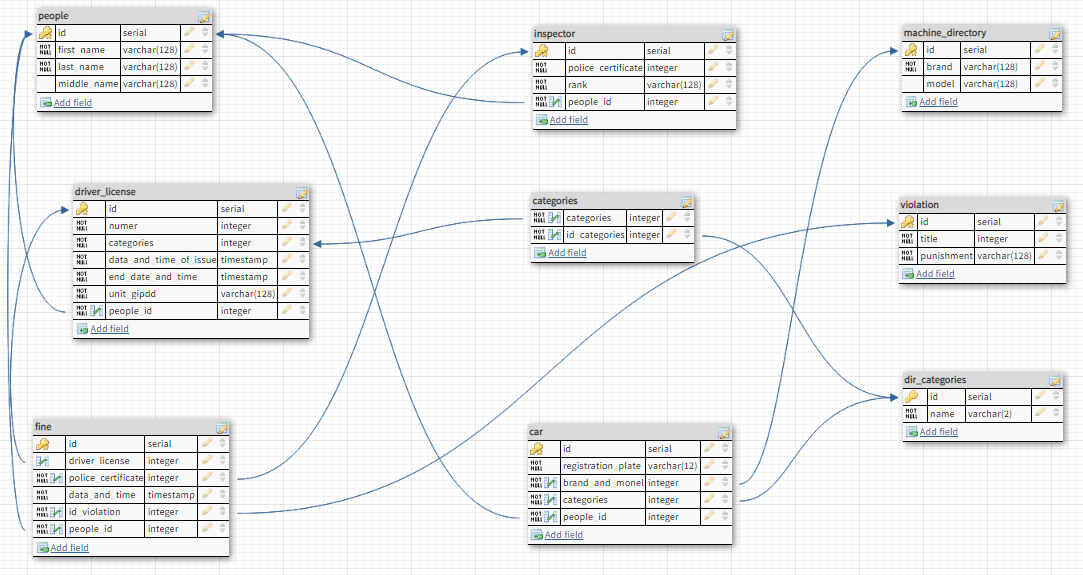
\includegraphics[scale=0.6]{../../diagram/diagram.png}
		\caption{Схема модели} 
		\label{pic:pic_name} % название для ссылок внутри кода
	\end{center}
\end{figure}

\section{Выводы}

В ходе выполнения работы была разработана ER-диаграмма модели данных, структура которой согласовывалась с преподавателем.

\end{document}
